\graphicspath{{images/}}

\section{Introduction}
\label{sec:introduction}

The bacterium \textit{Eschericia coli} and yeast \textit{Saccharomyces
  cerevisiae} are unicellular organisms studied as a model prokaryote
and eukaryote respectively.
% Compared to other species bacteria and yeasts have small compact genomes.
Much of their genomes have been conserved in other species over
billions of years of evolution
\citep{OBrien2005inparanoid}. \textit{S.~cerevisiae} was the first
eukaryote to have its entire genome sequenced \citep{goffeau1996life},
and is commonly used as a basis for the study of other eukaryotes
including human cells.

Bacteria and yeasts grow in colonies. In favourable conditions, growth
is exponential, and growth rate is a major component of fitness;
faster growing strains quickly come to dominate populations. At a
certain point, growth becomes limited and a stationary phase is
reached, so pressure also exists to use resources efficiently. In
short, fitness is governed by competing pressures on growth rate and
yield \citep{dethlefsen2007performance}. The fitness of microbes can
therefore be estimated from observations of growth
\citep{Baryshnikova2010,Addinall2011}. Cell cultures are commonly
grown on either the surface of a nutrient rich solid agar, or
suspended in a liquid mixture containing nutrients. To observe growth,
cultures are incubated and cell density is measured over
time. Identical strains might grow differently between mediums causing
fitness estimates to differ \citep{Baryshnikova2010}. Here, I focus on
estimating the fitness of microbes grown on a solid agar surface.

% The bacterium \textit{Eschericia coli} and yeast \textit{Saccharomyces
%   cerevisiae} are unicellular organisms studied as a model prokaryote
% and eukaryote respectively.
% Bacteria and yeasts grow in
% colonies. In favourable conditions, growth is exponential and this
% makes growth rate a major component of fitness; colonies of faster
% growing strains quickly come to dominate populations. At a certain
% point growth becomes limited and a stationary phase is reached. In
% short, fitness is governed by competing pressures on fast growth rate
% and yield \citep{dethlefsen2007performance}.
% Compared to other species bacteria and yeasts have small compact
% genomes. Many genes have been conserved in other species over billions
% of years of evolution
% \citep{OBrien2005inparanoid}. \textit{S.~cerevisiae} was the first
% eukaryote to have its entire genome sequenced \citep{goffeau1996life}
% and is particularly useful as a model of other eukaryotes such as
% human cells.

% The growth rate of microbial organisms is measurable and is often used
% to determine fitness (see~e.g.~\citet{Addinall2011}). In growth
% experiments, cell cultures are commonly grown in one of two types of
% medium: on the surface of a nutrient rich solid agar or in a liquid
% mixture containing nutrients. In both cases cultures are incubated and
% cell density is measured over time. Identical strains can grow
% differently in these environments and disagreement in fitness
% estimates has been observed \citet{Baryshnikova2010}. Here, I focus on
% estimating the fitness of microbes growing on solid agar surfaces.

%%% Genetic interaction, SGA and QFA %%%

Fitness estimates can be used to infer genetic interaction or drug
response. Using high-throughput methods, this can be conducted on a
genome-wide scale \citep{Costanzo2010,Andrew2013}. In a typical
genetic interaction screen, a strain is made with a background
mutation in a query gene. Double mutants are created by introducing a
second deletion to this strain. Genetic interactions are inferred by
comparing the growth of double mutants with controls containing a
neutral background mutation (effectively single mutants). If the
double mutant is fitter than predicted given the observations of
control fitness, then the deletion is said to suppress the defect of
the query mutation. If the double mutant is less fit than predicted
given the observations of control fitness, then the deletion is said
to enhance the defect of the query mutation. Either scenario suggests
that the two genes interact. Due to redundancy, single deletions are
often non-lethal. This allowed \citet{Costanzo2010} to explore genetic
interactions for \(\sim\)75\% of the \textit{S. cerevisiae} genome.

% One %

Synthetic Genetic Array (SGA) and Quantitative Fitness Analysis (QFA)
are high-throughput fitness-screening methods, which use solid agar,
and make quantitative estimates of microbial fitness
\citep{Baryshnikova2010sga,Banks2012}. In SGA, cultures are pinned
onto plates. Typically, in QFA, dilute liquid cultures are inoculated
onto plates. In both procedures, cultures are arranged in rectangular
arrays. Each culture is a single strain and each plate my may contain
100s or 1000s of different strains. Whole genomes can be explored
using different combinations of query genes and deletions. I study
QFA, in which a model is fit to growth curves, and fitness estimates
are defined in terms of model parameters. Typical QFA procedures use
16x24 arrays (384 spots). In contrast, SGA procedures use a single
endpoint assay of culture area to quantify growth, and, typically, use
larger 32x48 arrays (1536 dots). In QFA, inoculum density may be
varied to capture more or less of the growth curve; the most dilute
cultures are inoculated with \(\sim\)100 starting cells
\citep{Addinall2011}. Plates are incubated at a controlled temperature
and periodically removed for whole plate photographs to be
taken. Incubation lasts several days, to capture both the exponential
and stationary growth phases. The software Colonyzer
\citep{Lawless2010} converts optical density measurements in
photographs to cell density timecourses for each culture. Past
analysis fit the logistic growth model (\ref{eq:logistic_model}). The
differential form and solution of the logistic model
\citep{Verhulst1845} are given in (\ref{eq:logistic_model}), where
\(C\) is cell density, \(r\) is a growth constant, and \(K\) is a
carrying capacity.
% Logistic model equations
\begin{subequations}
  \label{eq:logistic_model}
  \begin{align}
    &\dot{C} = rC\left(1 - \frac{C}{K}\right)\\
    &C(t) = \frac{KC(0)e^{rt}}{K + C(0)(e^{rt}-1)}
  \end{align}
\end{subequations}
%
The logistic model is a simple mechanistic model describing
self-limiting growth and has a sigmoidal solution. Growth begins
exponentially, with rate \(rC\), and curtails as the population size
increases and cells begin to compete for some limited resource. Cell
density reaches a final carrying capacity, \(K\), at the stationary
phase. In QFA, nutrients must diffuse through agar to reach cells
growing on the surface. \(K\) might be reached when nutrients run out,
or growth becomes diffusion limited and is approximately
stationary. Fitting the logistic model to a 384 culture plate,
requires culture level parameters for \(r\) and \(K\), and either
plate or culture level parameters for \(C(0)\), making a total of 769
or 1152 parameters.

The growth constant \(r\) could be used as a fitness measure.
\citet{Addinall2011}, however, define a more complicated fitness
measure as the product of Maximum Doubling Rate (MDR) and Maximum
Doubling Potential (MDP), which they calculate from logistic model
parameters. MDR is the doubling rate at the beginning of the
exponential growth phase. MDP is the average number of cell divisions
between inoculation and stationary phase.
%
\begin{subequations}
  \label{eq:MDR_MDP}
    \begin{align}
      MDR &= \frac{r}{log\left(\frac{2(K-C(0))}{K-2C(0)}\right)}\\
      MDP &= \frac{log\left(\frac{K}{C(0)}\right)}{log(2)}
    \end{align}
\end{subequations}
%
To improve the quality of fits, QFA now uses the generalised logistic
model which requires an extra shape parameter for each culture
\citep{Banks2012}. Standard and generalised logistic model \(r\) are
not equivalent, so comparison relies on MDR and MDP as fitness
measures. Either model can be fit using the QFA \textsf{R} package
\citep{qfa2016}.
% //Could remove//\citet{Addinall2011} used QFA and
% \textit{S. cerevisiae} to screen for genes involved in telomere
% stability which is related to ageing and cancer and has implications
% for human health and disease. Hits from this study have been
% successfully followed to discover new biology
% \citep{Holstein20141259}. (To be honest I have no idea about the
% significance of what they found in this paper. We had a more general
% focus. If I have room I should probably try and sell the potential
% benefits and past successes of QFA a bit more to expand the
% motivation. Obviously I will mention the Addinall paper when I
% describe p15 in the methods.)  //Could remove//
% Example use of QFA by Addinall \citep{Addinall2011} telomeres.
% And follow up Holstein and Clark \citep{Holstein20141259}
%
\begin{Figure}
  \centering
  \includegraphics[width=\linewidth]{p15_section/p15_section_4x5_5_18}
  \captionof{figure}{\textbf{4x5 section of a QFA plate (P15).}
    Cropped from a 16x24 format solid agar plate inoculated with
    dilute \textit{S. cerevisiae} cultures. Image captured after
    \(\sim\)2.5 days incubation at 27\(^{\circ}C\).}
  \label{fig:p15_section}
\end{Figure}
%
Since QFA aims to differentiate strains by fitness, many different
strains are grown on one plate, and fast and slow growing strains
often grow side-by-side. This is exemplified in
Figure~\ref{fig:p15_section}, which shows a section of a QFA plate
from \citet{Addinall2011}. Cultures were inoculated with approximately
equal cell density, but grew to different sizes, at different
rates. In timecourses from this plate, all cultures appear to reach
the stationary phase at a similar timepoint, despite starting with the
same amount of nutrients and growing at different rates. This suggests
a global growth-limiting effect, which might be caused by an
interaction between cultures. I test whether the interaction is a
competition effect, caused by diffusion of nutrients along gradients
formed between fast and slow growing neighbours. Competition has
implications for growth estimates; growth will appear faster or slower
for each neighbour, than it would if cultures grew independently. The
experiment in Figure~\ref{fig:stripes_images} provides further
evidence of an interaction between neighbours. Identical strains were
repeated in the same positions on two plates, but on one plate every
second column was left empty. Cultures in
Figure~\ref{fig:stripes_images}a, with fewer neighbours, grew larger
%(how much? I can look at the data myself) **
than the same cultures in Figure~\ref{fig:stripes_images}b.

Neighbour interactions might be affecting fitness estimates. Current
QFA analysis, using the logistic model, assumes that cultures grow
independently. A sigmoidal curve fits QFA data poorly in many cases.
%% evidence? **
I aim to correct for competition using a network model of nutrient
diffusion and nutrient-dependent growth, to improve the fit of
individual growth curves, and increase the accuracy and precision of
fitness estimates.
\begin{Figure}
  \centering
  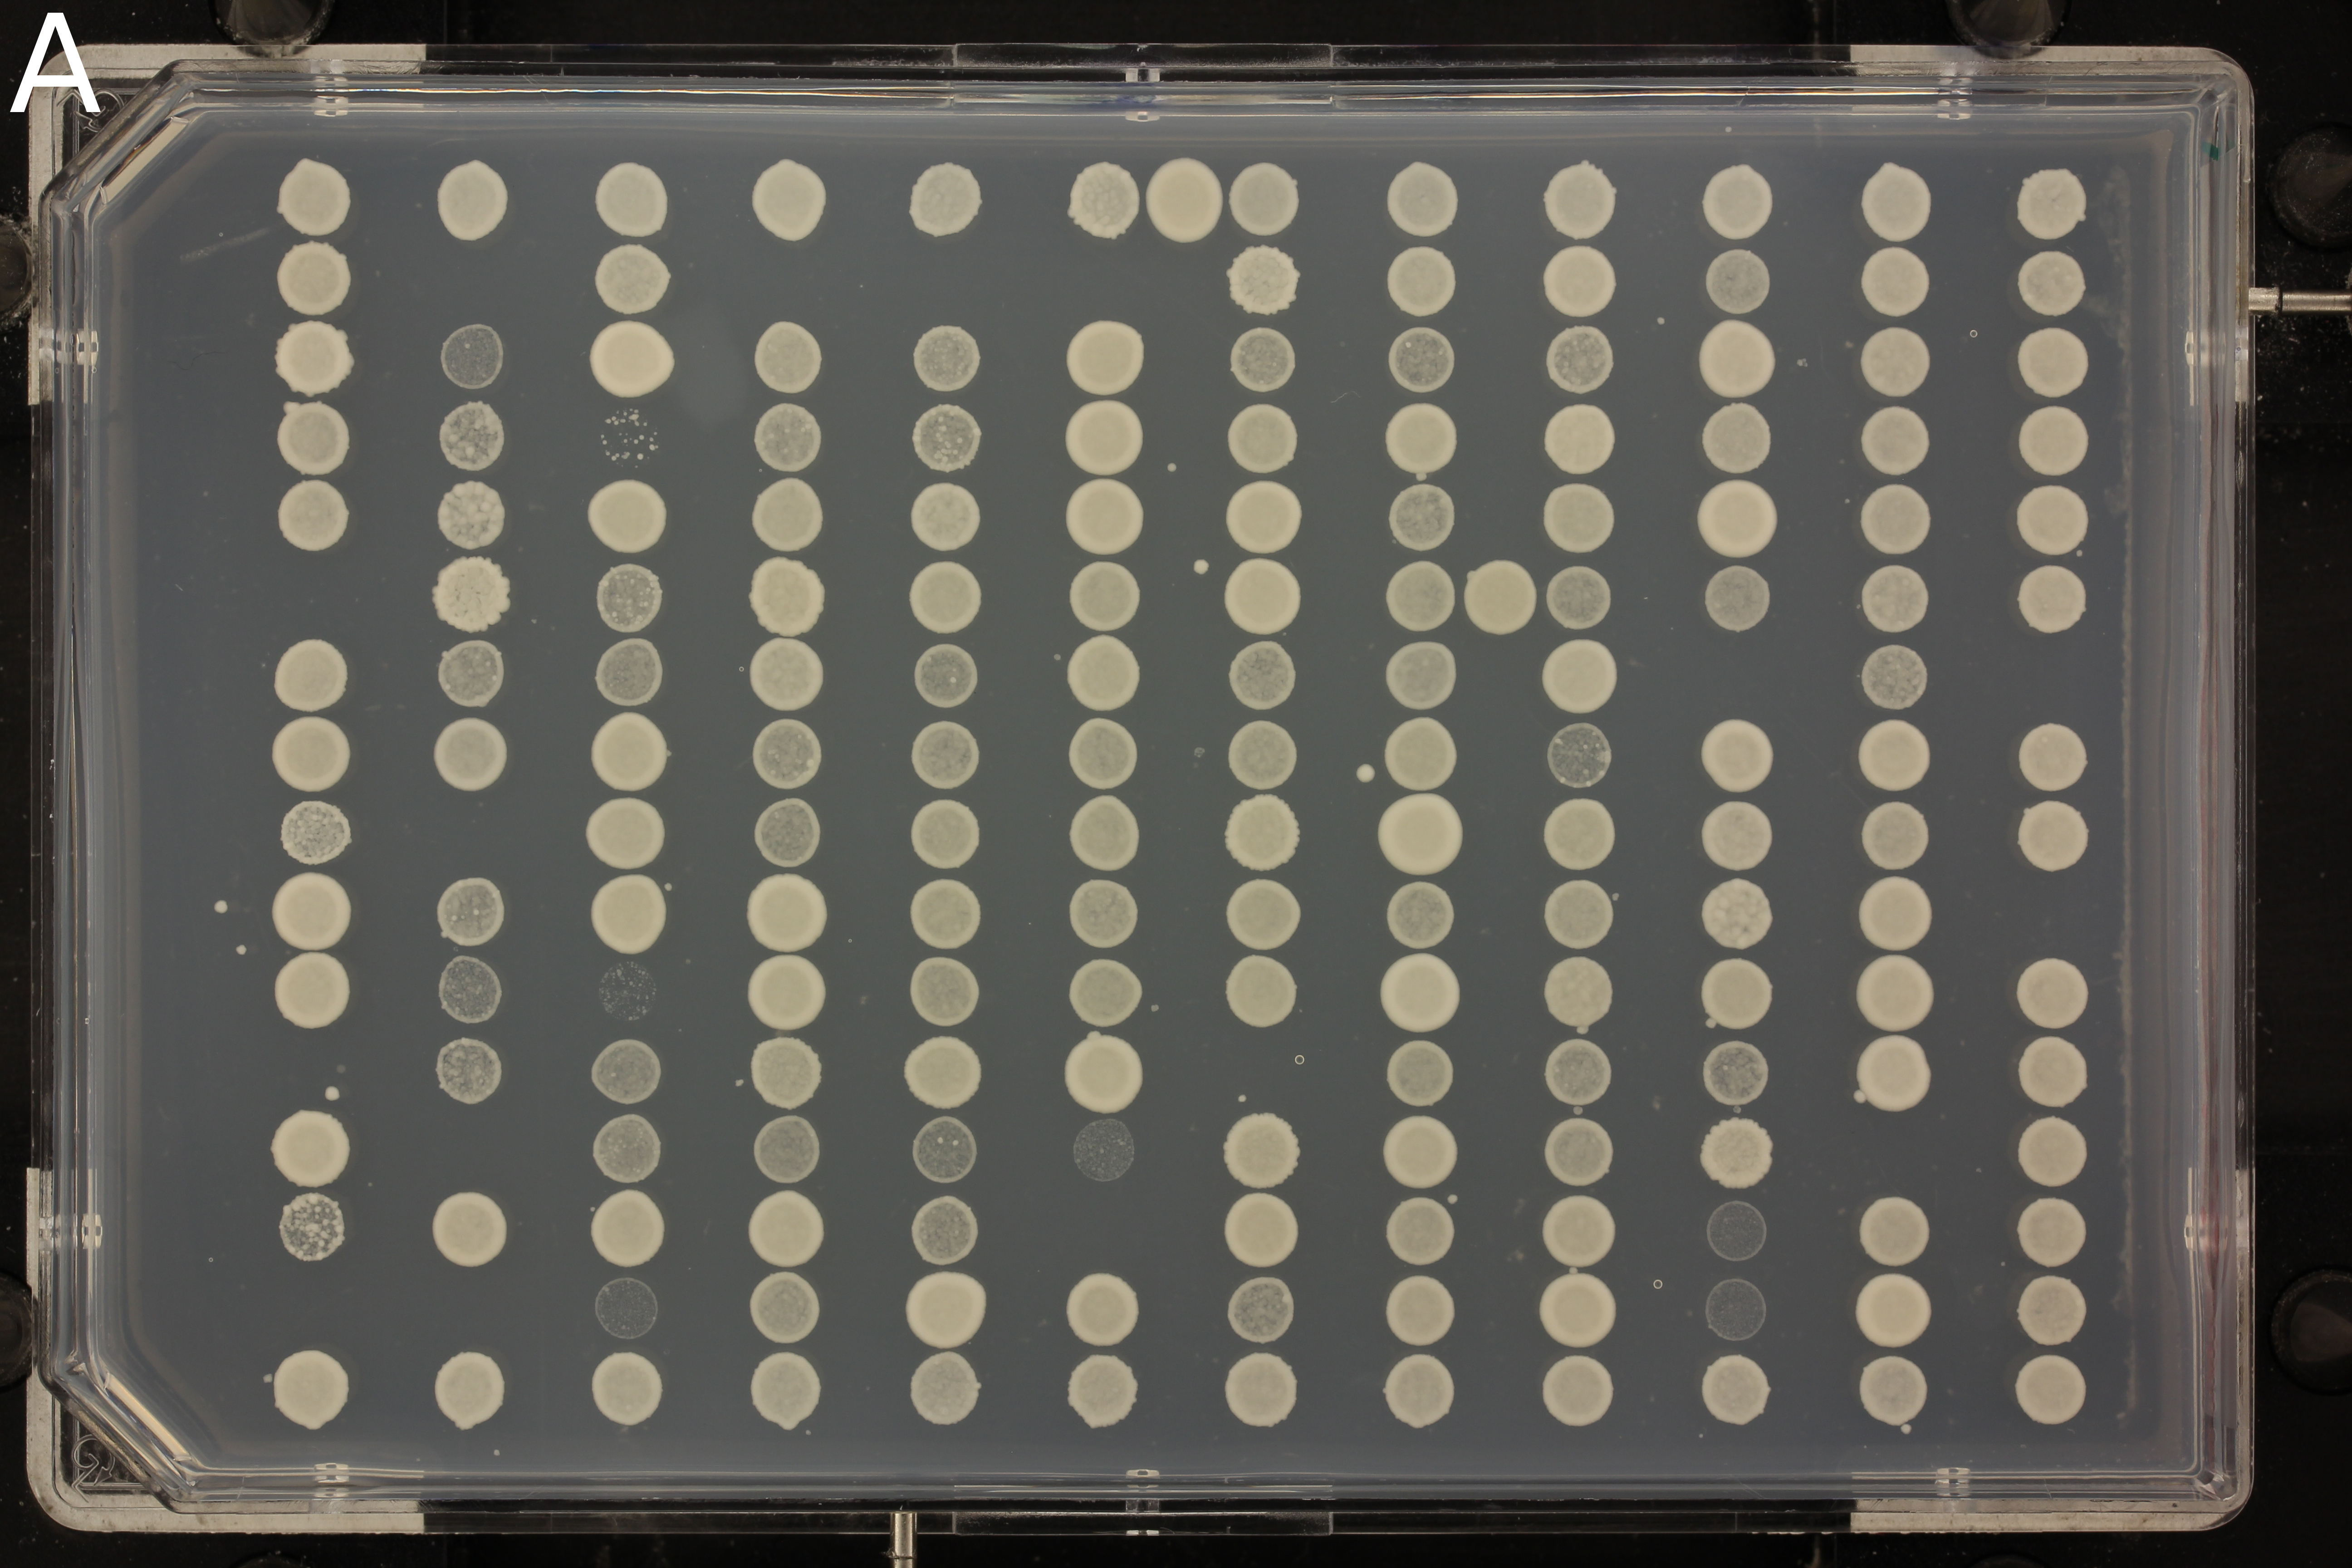
\includegraphics[width=\linewidth]{stripes/final/striped_A}
  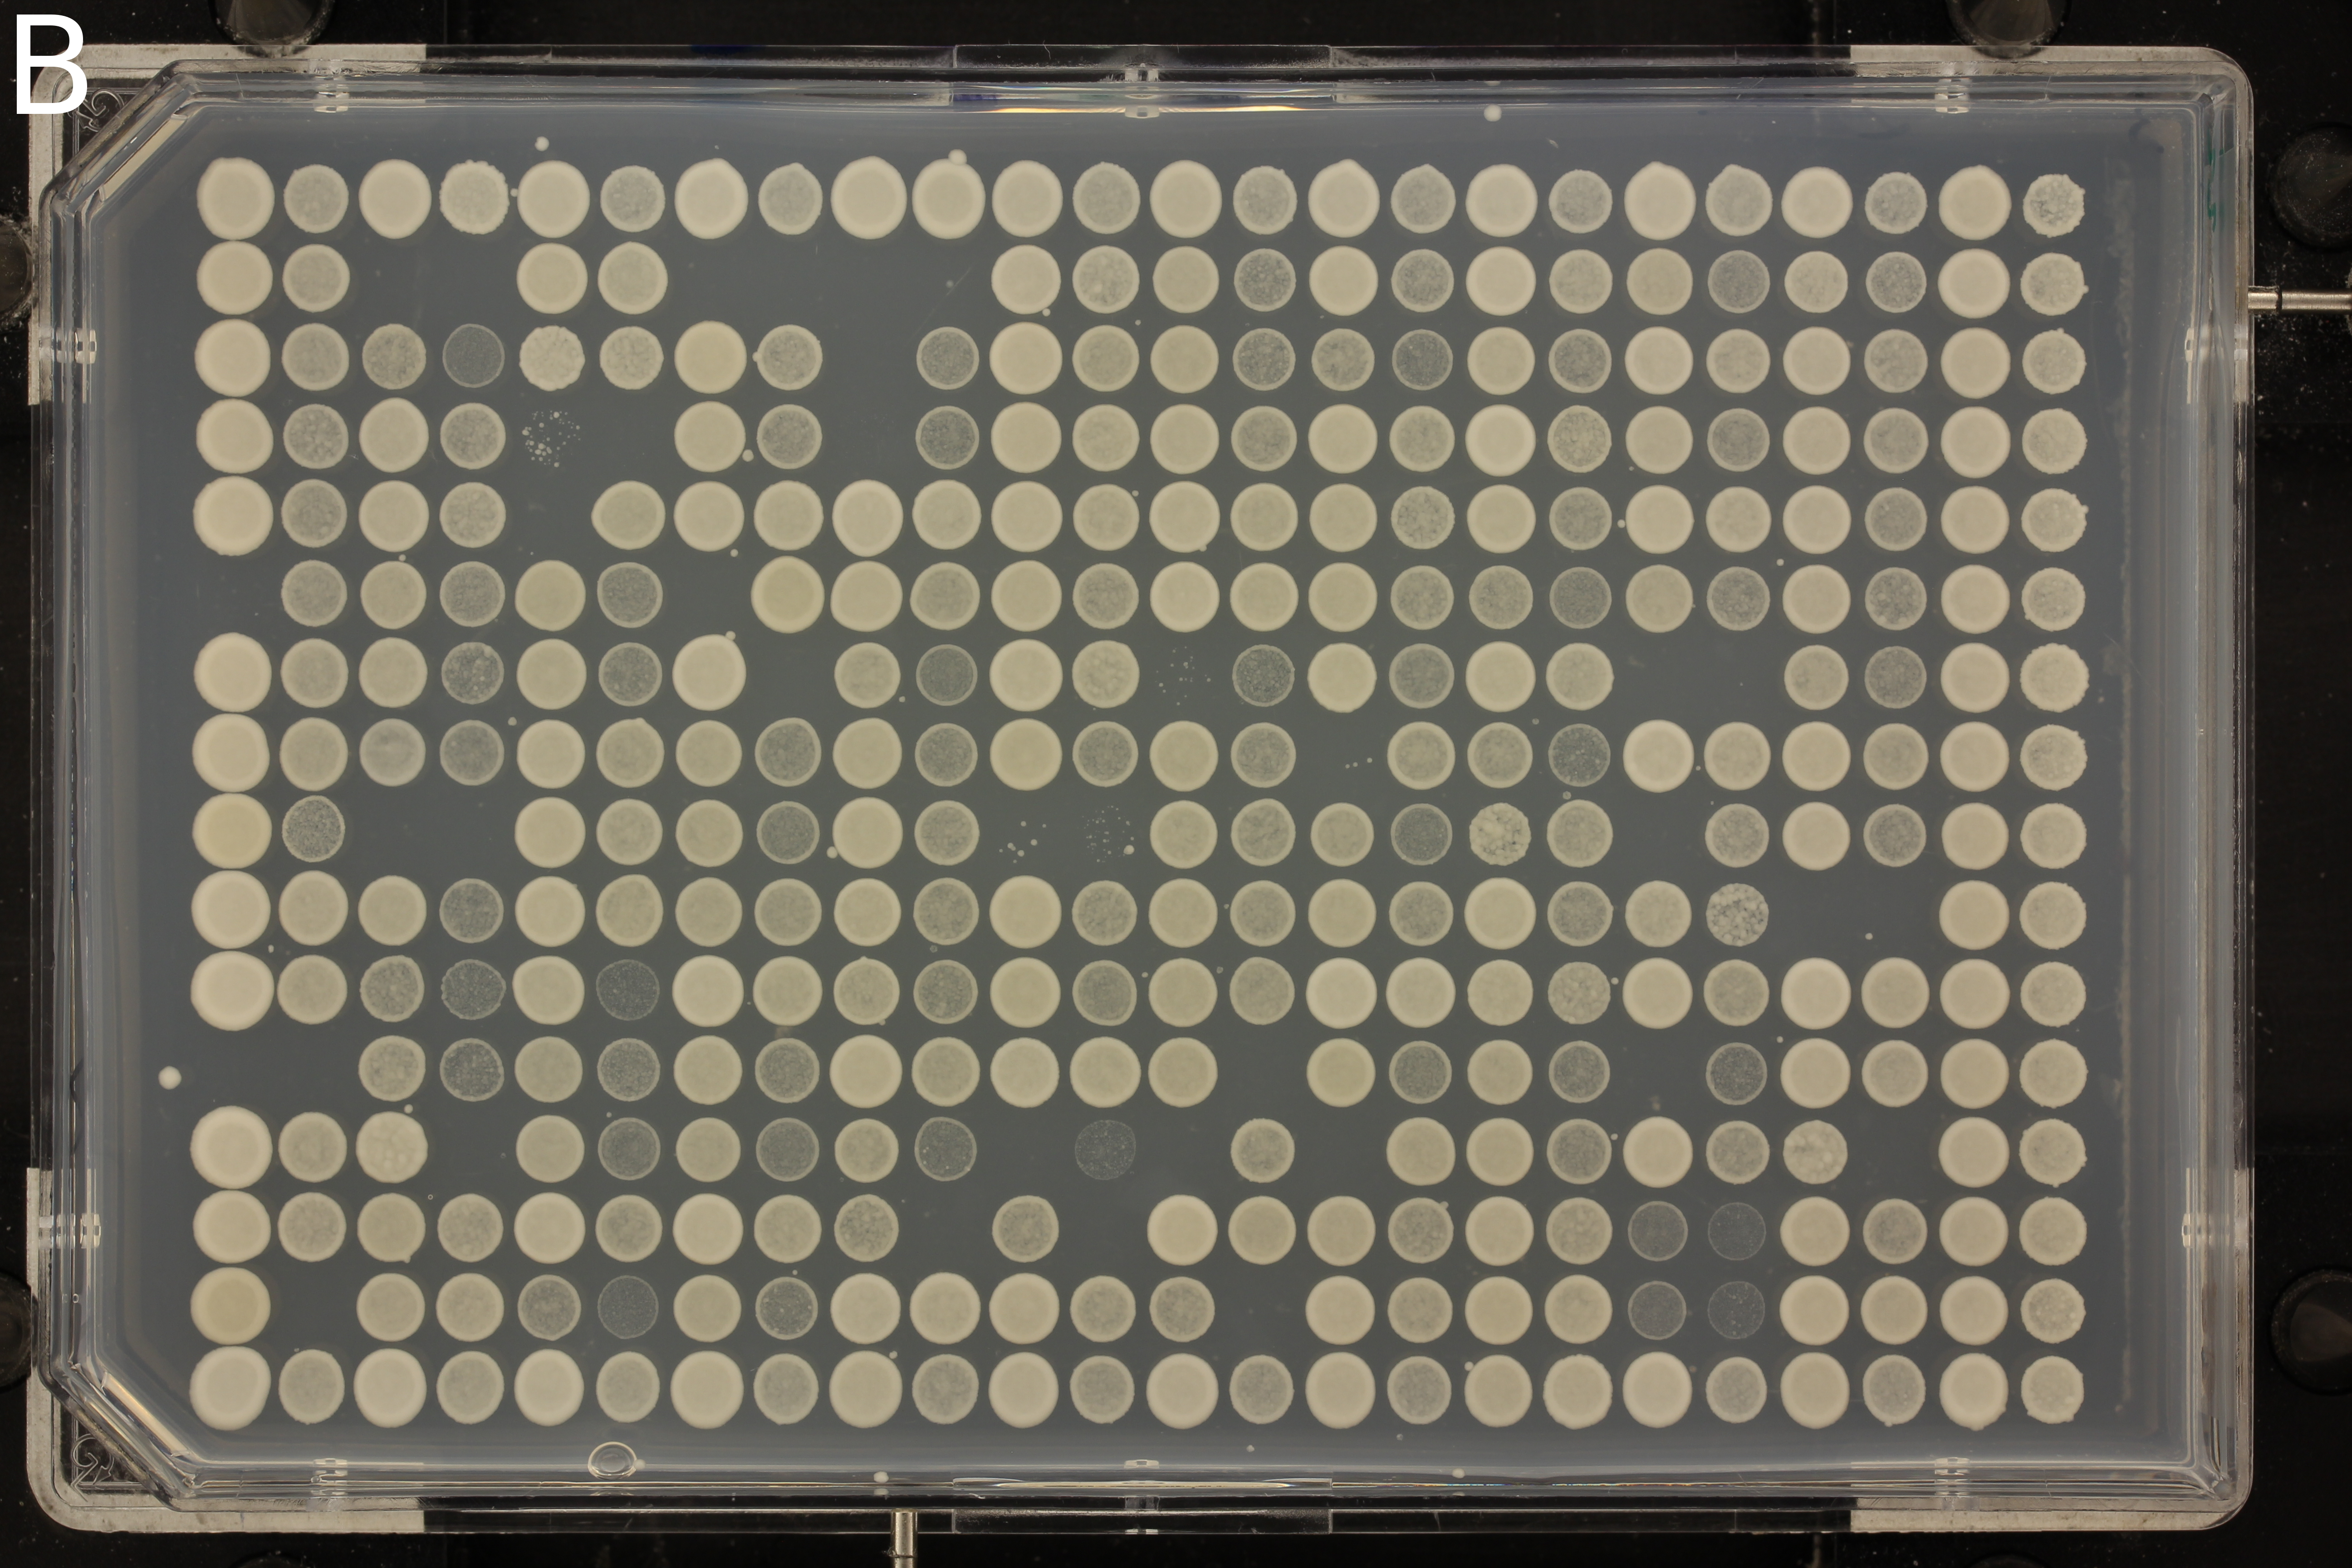
\includegraphics[width=\linewidth]{stripes/final/filled_B}
  \captionof{figure}{\textbf{Plates from a QFA experiment designed to
      examine competition.}  A) ``Stripes'' plate; B) ``Filled''
    plate. Identical strains are repeated in the same postition on
    each plate, except for in every 2nd column in A, where locations
    are left empty. The extra columns in B are a transposition of the
    columns to the left, but with a different query mutation. The
    leftmost column in B contains repeats of a control with a neutral
    deletion. Cultures were inoculated with a higher cell density than
    in Figure~\ref{fig:p15_section}.
    % A) The ``Stripes'' plate inocluated with a more concentrated
    % \textit{S. Cerevisiae} inoculum (no cells inocluated on alternate
    % columns). B) ``Filled'' plate: Same as in A, but with strains of
    % similar growth rate inoculated in the positions missing in A.
  }
  \label{fig:stripes_images}
\end{Figure}
%
There have been attempts to reduce and correct for competition effects
experimentally and statistically. This does not require explicit
knowledge or modelling of the source of interaction. QFA data for edge
cultures is noisy due to reflections from plate edges. This is only
partially corrected for by Colonyzer \citep{Lawless2010}. As a result,
data for edge cultures is usually discarded. \citet{Addinall2011} grow
repeats of a neutral deletion in edge locations, rather than leave
them empty, because of concerns about competition. Plates could also
be repeated with randomised culture positions. However, this is
unlikely to remove all bias; for instance, the fastest growing strains
would always have slower growing neighbours. In an SGA study,
\citet{Baryshnikova2010} use various statistical techniques to improve
the correlation between repeats of the same strain in different
positions. I expect that an explicit model of competition, fit to
whole growth curves, will provide a better correction and improve
fitness estimates, without requiring extra repeats. Furthermore, a
model might identify and explain the source of
competition. Simulations of a successful model could be used, not only
to analyse existing data, but to compare experimental designs, and
predict ways to reduce competition experimentally. Poisoning of
cultures by a signal molecule, such as ethanol, which
\textit{S. cerevisiae} produces in the metabolism of sugars by
fermentation, is another possible source of interaction.
%%%% Quorum Sensing %%%%
QFA does not measure nutrients or signal, so, if more than one type of
interaction is significant, it will be very difficult to fit a
model. In such circumstances, experimental and statistical methods
might be the best approach.

% //Diffusion Equation: I am probably going to have to repeat this
% when I get to the discussion so I could just leave until then.//
% Previous model of nutrient diffusion.
\citet{Reo2014} use a 2D diffusion equation model to simulate nutrient
dependent growth of a single bacterial culture on a pertri dish. They
create a sink for nutrients from culture growth, and equate the flux
of nutrients through culture area with the rate of increase in culture
size. They keep culture density constant and allow culture area to
vary. This model could be adapted for QFA, if instead, culture area is
approximated as constant and culture density is allowed to vary. It
would, however, be too computationally intensive to fit such a model
to a full QFA plate in three-dimensions, especially if the model is to
be used to analyse many plates from high-throughput
experiments. Therefore, a simpler model of nutrient diffusion is
required.
%//Diffusion Equation//P

Lawless proposes a network model of nutrient diffusion and
nutrient-dependent growth (Figure~\ref{fig:comp_model_schematic}),
hereinafter the competition model, which uses reaction equations and a
mass action kinetic approximation.
% (\ref{eq:reaction},\ref{eq:competition_model})
Nutrient-dependent division of cells is represented by the reaction
equation,
\begin{equation}
  \label{eq:reaction}
    C + N \xrightarrow[]{b} 2C,
\end{equation}
where \(C\) is a cell, \(N\) is the amount of some limiting nutrient
required for one cell division, and \(b\) is a rate constant for the
reaction. The identity of \(N\) is unknown, but possible candidates
are sugar and nitrogen. Each culture, indexed i, has a separate
reaction (3) with growth constant \(b_{i}\). Mass action kinetics
gives the rate equation (\ref{eq:competition_model}a) for the amount
of cells, \(C_{i}\), in a culture, and the first term in the rate
equation (\ref{eq:competition_model}b) for the amount of nutrients,
\(N_{i}\), associated with a culture.
\begin{subequations}
  \label{eq:competition_model}
  \begin{align}
         % \frac{dC_{i}}{dt}& = b_{i}N_{i}C_{i},\\
         % \frac{dN_{i}}{dt}& = - b_{i}N_{i}C_{i} - k\sum_{j \epsilon \delta_i}(N_{i} - N_{j}).
         \dot{C_{i}}& = b_{i}N_{i}C_{i},\\
         \dot{N_{i}}& = - b_{i}N_{i}C_{i} - k\sum_{j \epsilon \delta_i}(N_{i} - N_{j}).
  \end{align}
      % \right\ Hello
      % \qquad
\end{subequations}
To arrive at the full competition model, the diffusion of nutrients
along gradients between a culture and its closest neighbours,
\(\delta_{i}\), is modelled by reactions of the form,
\begin{equation}
  \label{eq:diffusion_reaction}
  \left.\begin{aligned}
  &N_{i} \xrightarrow[]{k} N_{j}
       \end{aligned}
 \right.
 \qquad \forall~j \in \delta_{i},
  % \begin{align}
  % \end{align}
\end{equation}
where \(k\) is a nutrient diffusion constant which is independent on
culture location. Using mass action kinetics, the sum of diffusion
reactions between a culture and its neighbours gives the second term
in (\ref{eq:competition_model}b).


% To arrive at the full competition model, the diffusion of nutrients
% along gradients between a culture and its closest neighbours,
% \(\delta_{i}\), is modelled by reactions of the form,
% \begin{equation}
%   \label{eq:diffusion_reaction}
%   \left.\begin{aligned}
%   &N_{i} \xrightarrow[]{k} N_{j}\\
%   &N_{j} \xrightarrow[]{k} N_{i}
%        \end{aligned}
%  \right.
%  \qquad \forall~j \in \delta_{i},
%   % \begin{align}
%   % \end{align}
% \end{equation}
% where \(k\) is a nutrient diffusion constant.

% is represented by the second term in
% (\ref{eq:competition_model}b), where \(k\) is a nutrient diffusion
% constant. This can also be expressed a series of reversible
% first-order reactions,
% \begin{equation}
%   \label{eq:diffusion_reaction}
%   \left.\begin{aligned}
%   &N_{i} \xrightarrow[]{k} N_{j}\\
%   &N_{j} \xrightarrow[]{k} N_{i}
%        \end{aligned}
%  \right.
%  \qquad \forall~j \in \delta_{i},
%   % \begin{align}
%   % \end{align}
% \end{equation}
% % \begin{equation}
% %   \label{eq:diffusion_reaction}
% %   \left.
% %     N_{i} \xrightleftarrow[k]{k} N_{j}\\
% %  \right.\qquad
% %     \forall~j \in \delta_{i},
% %   % \begin{align}
% %   % \end{align}
% % \end{equation}
% and modelled with mass action kinetics.
Unlike the logistic model~(\ref{eq:logistic_model}), the competition
model has no analytical solution; instead, it must be solved
numerically. When \(k\) is set to zero, however, the competition model
reduces to the mass action equivalent of the logistic model,
hereinafter the mass-action logistic model, and has the same sigmoidal
solution. In this limit, parameters of the competition model can be
expressed in terms of parameters the logistic model (see
Section~\ref{sec:parameter_conversion}).

%%%% could go to methods %%%%
In QFA, \(C_{i}\) are observed and \(N_{i}\) are hidden. Inoculum
densities, \(C_{i}(0)\), are often below detectable levels. When
fitting the competition model, I assume that inoculum density is the
same for all cultures, nutrients are evenly distributed throughout the
agar at time zero, and \(k\) is constant across the plate. I can
therefore infer \(C(0)\), \(N(0)\), and \(k\) at the plate
level. Including growth constants, \(b_{i}\), for each of 384 cultures
on a typical plate, makes 387 parameters in total. The competition
model has roughly half as many parameters as the standard logistic
model, and a third as many as the generalised logistic model.
%%%%%%%%%%%%%%%%%%%%%%%%%%%%%%%
\begin{Figure}
  \centering
  \includegraphics[width=\linewidth]{comp_model/comp_model_schematic2}
  \captionof{figure}{\textbf{Schematic of the competition model.}
    Cultures, represented by circles indexed i, grow in a rectangular
    array on the surface of a nutrient containing solid agar. The agar
    is divided into equal areas surrounding each culture. Each culture
    has an amount of cells, \(C_{i}\), and is associated with an
    amount of nutrients, \(N_{i}\). Arrows represent diffusion of
    nutrients between cultures. Darker blue circles, \(\delta_{i}\),
    are the closest neighbours of the red culture, \(i\).}
  \label{fig:comp_model_schematic}
\end{Figure}

% Now I am justifying some assumptions %%
The competition model makes many other approximations. It is a
deterministic model which uses a continuum approximation for numbers
of reactant species. In QFA, populations begin with \(\sim\)100 cells,
but quickly grow to reach thousands of cells, so this approximation
appears valid. Mass action kinetics applies to reactions in a well
stirred mixture, and is, perhaps, less valid for cultures growing on
solid agar. A mass action approximation has, nevertheless, been
successful in other situations where this assumption is questionable:
in the Lotka-Volterra model of predator-prey dynamics
\citep{Berryman1992} and in signalling and reaction models inside
cells \citep{Aldridge2006,Chen2010}. The order of a reaction also
affects the rate equation, but the identity, and quantity of the
nutrient molecule is unknown. Reactions also assume that all nutrients
are converted to cells and include no model of metabolism. I justify
the use of the competition model because in the independent limit it
has the same solution as the logistic model, long used to model
microbial growth. Furthermore, collectively fitting the competition
model involves a large number of parameters and data points, and will
require many simulations to be run. Computational feasibility
necessitates the use of many approximations.

% For an example of a successful QFA study and follow up using the
% logistic model see \citet{Addinall2011} and
% \citet{Holstein20141259}.

% The competition model might estimate more accurate and precise growth
% parameters and fitnesses. Doing so will increase the power to infer
% genetic interaction and drug response which could lead to further
% discoveries. For an example of a successful QFA study and follow up
% using the logistic model see \citet{Addinall2011} and
% \citet{Holstein20141259}.

% Comment on all nutrients go to cells can wait until methods
% % Fractal kinetics can wait until the discussion.
% fractal kinetics if nutrient diffusion is limited inside cultures, due
% to gel-like properties of the medium \citep{savageau1995,Kopelman1988}
% \citep{savageau1995,Kopelman1988}

%%% Local Variables:
%%% mode: latex
%%% TeX-master: "report"
%%% End:
